% Requires \usepackage{pgfplots} (\pgfplotsset{compat=1.18}) in the preamble
\begin{figure}[htbp]
\centering
\begin{minipage}[t]{0.48\textwidth}
  \centering
  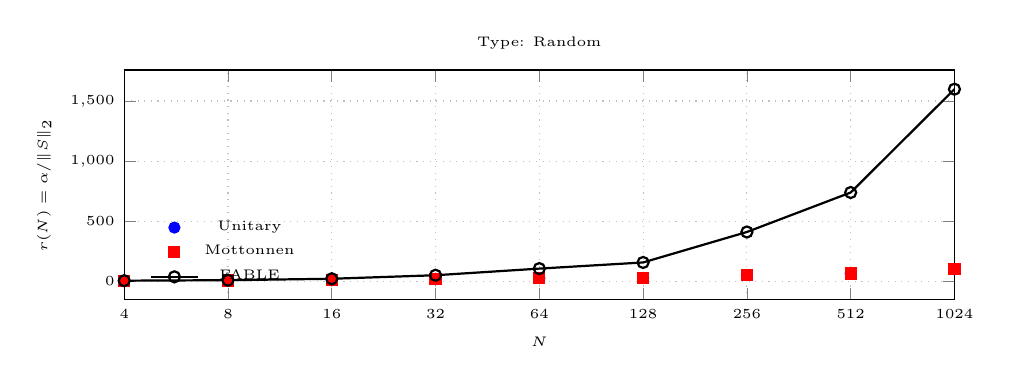
\begin{tikzpicture}
  \begin{axis}[
      width=\linewidth,
      height=4.5cm,
      xmode=log,
      log basis x=2,
      xmin=4, xmax=1024,
      xtick={4,8,16,32,64,128,256,512,1024},
      xticklabels={4,8,16,32,64,128,256,512,1024},
      xlabel={$N$},
      ylabel={$r(N) = \alpha / \|S\|_2$},
      xlabel near ticks,
      ylabel near ticks,
      xlabel style={font=\tiny},
      ylabel style={font=\tiny},
      title style={font=\tiny, yshift=-2pt},
      tick label style={font=\tiny},
      grid=both,
      grid style={dotted},
      minor tick num=0,
      enlarge x limits=false,
      title={Type: Random},
      legend style={
          font=\tiny,
          draw=none,
          fill=none,
          at={(0.02,0.02)},
          anchor=south west,
      },
  ]

  % --- Unitary ---
  \addplot[blue, only marks, mark=*, mark size=2pt] coordinates {
  (4, 4.923125e+00) (8, 6.434595e+00) (16, 1.047928e+01) (32, 1.778668e+01) (64, 2.638206e+01) (128, 2.768144e+01) (256, 5.127784e+01) (512, 6.530255e+01) (1024, 9.991375e+01) 
  };
  \addlegendentry{Unitary}

  % --- Mottonnen ---
  \addplot[red, only marks, mark=square*, mark size=2pt] coordinates {
  (4, 4.923125e+00) (8, 6.434595e+00) (16, 1.047928e+01) (32, 1.778668e+01) (64, 2.638206e+01) (128, 2.768144e+01) (256, 5.127784e+01) (512, 6.530255e+01) (1024, 9.991375e+01) 
  };
  \addlegendentry{Mottonnen}

  % --- FABLE reference ---
  \addplot[black, thick, mark=o] coordinates {
  (4, 4.923125e+00) (8, 9.099891e+00) (16, 2.095855e+01) (32, 5.030832e+01) (64, 1.055283e+02) (128, 1.565899e+02) (256, 4.102228e+02) (512, 7.388140e+02) (1024, 1.598620e+03) 
  };
  \addlegendentry{FABLE}

  \end{axis}
  \end{tikzpicture}
  \vspace{0.3cm}

  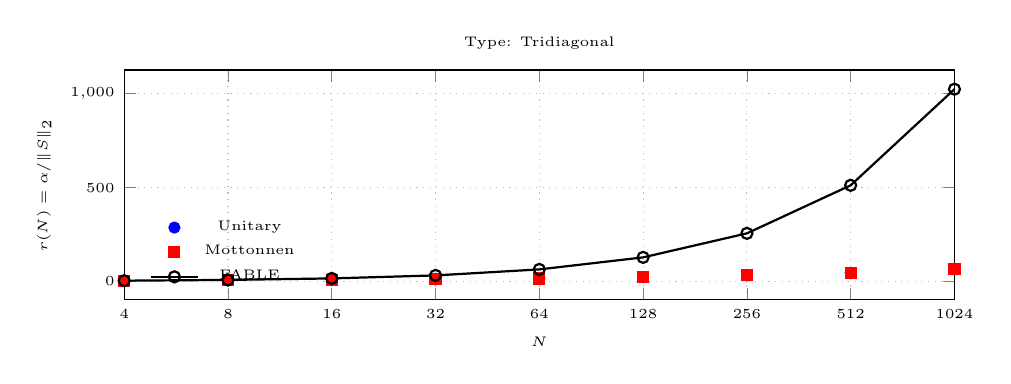
\begin{tikzpicture}
  \begin{axis}[
      width=\linewidth,
      height=4.5cm,
      xmode=log,
      log basis x=2,
      xmin=4, xmax=1024,
      xtick={4,8,16,32,64,128,256,512,1024},
      xticklabels={4,8,16,32,64,128,256,512,1024},
      xlabel={$N$},
      ylabel={$r(N) = \alpha / \|S\|_2$},
      xlabel near ticks,
      ylabel near ticks,
      xlabel style={font=\tiny},
      ylabel style={font=\tiny},
      title style={font=\tiny, yshift=-2pt},
      tick label style={font=\tiny},
      grid=both,
      grid style={dotted},
      minor tick num=0,
      enlarge x limits=false,
      title={Type: Tridiagonal},
      legend style={
          font=\tiny,
          draw=none,
          fill=none,
          at={(0.02,0.02)},
          anchor=south west,
      },
  ]

  % --- Unitary ---
  \addplot[blue, only marks, mark=*, mark size=2pt] coordinates {
  (4, 3.887007e+00) (8, 5.656112e+00) (16, 8.000000e+00) (32, 1.131371e+01) (64, 1.600000e+01) (128, 2.262742e+01) (256, 3.200000e+01) (512, 4.525483e+01) (1024, 6.400000e+01) 
  };
  \addlegendentry{Unitary}

  % --- Mottonnen ---
  \addplot[red, only marks, mark=square*, mark size=2pt] coordinates {
  (4, 3.887007e+00) (8, 5.656112e+00) (16, 8.000000e+00) (32, 1.131371e+01) (64, 1.600000e+01) (128, 2.262742e+01) (256, 3.200000e+01) (512, 4.525483e+01) (1024, 6.400000e+01) 
  };
  \addlegendentry{Mottonnen}

  % --- FABLE reference ---
  \addplot[black, thick, mark=o] coordinates {
  (4, 3.887007e+00) (8, 7.998950e+00) (16, 1.600000e+01) (32, 3.200000e+01) (64, 6.400000e+01) (128, 1.280000e+02) (256, 2.560000e+02) (512, 5.120000e+02) (1024, 1.024000e+03) 
  };
  \addlegendentry{FABLE}

  \end{axis}
  \end{tikzpicture}
\end{minipage}
\hfill
\begin{minipage}[t]{0.48\textwidth}
  \centering
  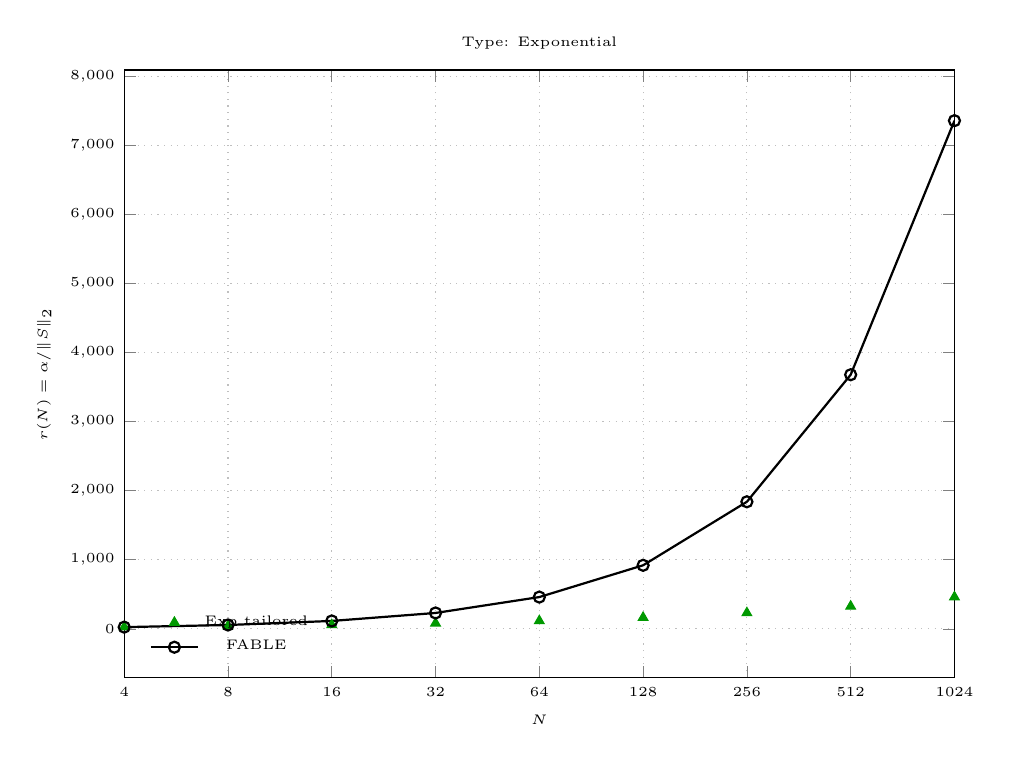
\begin{tikzpicture}
  \begin{axis}[
      width=\linewidth,
      height=9.3cm,
      xmode=log,
      log basis x=2,
      xmin=4, xmax=1024,
      xtick={4,8,16,32,64,128,256,512,1024},
      xticklabels={4,8,16,32,64,128,256,512,1024},
      xlabel={$N$},
      ylabel={$r(N) = \alpha / \|S\|_2$},
      xlabel near ticks,
      ylabel near ticks,
      xlabel style={font=\tiny},
      ylabel style={font=\tiny},
      title style={font=\tiny, yshift=-2pt},
      tick label style={font=\tiny},
      grid=both,
      grid style={dotted},
      minor tick num=0,
      enlarge x limits=false,
      title={Type: Exponential},
      legend style={
          font=\tiny,
          draw=none,
          fill=none,
          at={(0.02,0.02)},
          anchor=south west,
      },
  ]

  % --- Exp_tailored ---
  \addplot[green!60!black, only marks, mark=triangle*, mark size=2pt] coordinates {
  (4, 2.426581e+01) (8, 3.891743e+01) (16, 5.684466e+01) (32, 8.104691e+01) (64, 1.148513e+02) (128, 1.625070e+02) (256, 2.298489e+02) (512, 3.250658e+02) (1024, 4.597161e+02) 
  };
  \addlegendentry{Exp\_tailored}

  % --- FABLE reference ---
  \addplot[black, thick, mark=o] coordinates {
  (4, 2.426581e+01) (8, 5.503756e+01) (16, 1.136893e+02) (32, 2.292353e+02) (64, 4.594052e+02) (128, 9.192785e+02) (256, 1.838791e+03) (512, 3.677699e+03) (1024, 7.355457e+03) 
  };
  \addlegendentry{FABLE}

  \end{axis}
  \end{tikzpicture}
\end{minipage}
\caption{Subnormalization ratio $r(N)=\alpha/\|S\|_2$ versus $N$, compared against FABLE.}
\label{fig:subnorm}
\end{figure}
